%========================================================================
% Modelo para elaboracao de textos academicos: TCC, dissertacoes e teses
% Elaborado pelo GISIS - Grupo de Imageamento Sismico e Inversao Sismica.
%========================================================================
\chapter{Resultados e Discussões}
\label{ch:resultados}

Neste capítulo, são apresentados os resultados da comparação entre os métodos de \citeonline{podvin1991finite}, \citeonline{jeong2008fast} e \citeonline{noble2014accurate} em termos de precisão no cálculo dos tempos de trânsito e desempenho computacional. Assim que apresentados, ambos recebem suas respectivas discussões individualmente.

A aplicação com modelo homogêneo replica o experimento realizado no trabalho de \citeonline{cai2023improved}, onde a inovação em precisão foi desenvolvida para o \textit{Fast Iterative Method}. A aplicação com modelo de duas camadas replica o experimento contido em \citeonline{alves2022refraction}. E a aplicação em modelo complexo mostra como os tempos de trânsito se comportam na presença de altos contrastes de velocidade e qual o tempo de execução para cada método no modelo mais realístico.    

\section{Aplicação em modelo homogêneo}

A Tabela \ref{table_homog} apresenta os tempos de execução, o erro médio e o erro máximo para cada formulação. Os resultados gerados utilizando a implementação de \citeonline{cai2023improved} foram executados no mesmo ambiente, segundo as configurações apresentadas no capítulo de Metodologia, devido a disponibilização do código publicamente.  

\begin{table}[H]
	\caption{Tempo de execução, erro médio e máximo em relação a equação analítica para meio homogêneo. Aplicação dos métodos utilizados relacionando com os resultados do experimento de \citeonline{cai2023improved}.}
	\begin{tabular}{r|ccc}
		\multicolumn{1}{c|}{} & Tempo {[}s{]} & Erro médio {[}s{]} & Erro máximo {[}s{]} \\ \hline
		\citeonline{podvin1991finite} & 0,9661        & 0,000273           & 0,000762            \\ \hline
		\citeonline{jeong2008fast}    & 0,6082        & 0,000837           & 0,001323            \\ \hline
		\citeonline{noble2014accurate}& 0,8085        & 0,000037           & 0,000069            \\ \hline
		\citeonline{cai2023improved}  & 1,9312        & 0,000196           & 0,000282           
	\end{tabular}
	\label{table_homog}
\end{table}

No teste do modelo homogêneo (Tabela \ref{table_homog}) nota-se a superioridade em performance do método de \citeonline{jeong2008fast}, porém os erros registrados são os mais altos em relação aos outros métodos testados. O método de \citeonline{cai2023improved} consegue reduzir o erro do \textit{Fast Iterative Method}, contudo, além de não ser o mais preciso entre os métodos analisados, a nova formulação demostrou performance inferior em relação às demais estudadas. O método que demonstrou mais precisão foi a nova implementação do \textit{Fast Sweeping Method} utilizando a estratégia de paralelização de \citeonline{detrixhe2013parallel} e os operadores desenvolvidos no trabalho de \citeonline{noble2014accurate}. A eficiência computacional do \textit{Fast Sweeping Method} não se destacou como a mais performática, porém se demonstra promissora ao considerar o conjunto entre precisão e performance.  

\section{Aplicação em modelo de refração}

As Figuras \ref{fig:general_refraction_study}, \ref{fig:precision_refraction_study} e \ref{fig:reciprocity_refraction_study} exibem todo o estudo de precisão com os tempos calculados da fonte para os receptores (tempos diretos) e dos receptores para a fonte (tempos recíprocos). As cores indicam os métodos, sendo o azul para a formulação de \citeonline{podvin1991finite}, o amarelo para a formulação de \citeonline{jeong2008fast} e o verde para a formulação de \citeonline{noble2014accurate}. Os estilos de linha representam o parâmetro de discretização, então, as linhas sólidas representam o modelo de 25 m, as linhas tracejadas, o de 50 m, e as linhas com ponto e traço, o de 100 m. 

\begin{table}[H]
	\caption{Tempo de execução para cada discretização e reciprocidade para o modelo de 25 m.}
	\begin{tabular}{r|cccc}
		& 100 m    & 50 m     & 25 m     & Reciprocidade \\ \hline
		\citeonline{podvin1991finite}   & 0,0676 s & 0,3141 s & 3,5324 s & 7896,2 s        \\ \hline
		\citeonline{jeong2008fast} & 0,0491 s & 0,0987 s & 0,6261 s & 921,8 s              \\ \hline
		\citeonline{noble2014accurate} & 0,1042 s & 0,2286 s & 0,8284 s & 1382,5 s          \\
	\end{tabular}
	\label{table_refModel}
\end{table}

A Tabela \ref{table_refModel} mostra, para cada método testado, um teste de escalabilidade, onde o domínio do problema cresce para verificar o desempenho computacional dos métodos numéricos. A análise de reciprocidade foi crucial para verificar extravasamentos de memória quando aplicadas múltiplas posições de tiro. A validação em aplicações de imageamento sísmico também pode ser observada a partir do estudo de reciprocidade, pois o tempo de execução importa na geração de resultados. 

A Figura \ref{fig:general_refraction_study} mostra a configuração de todos os métodos para o tiro central, sendo o tempo analítico a linha sólida de cor preta. A Figura \ref{fig:precision_refraction_study} mostra a ordem do erro para cada método e a Figura \ref{fig:reciprocity_refraction_study} mostra as diferenças entre o tempo direto e recíproco para cada método utilizando o modelo de duas camadas com 25 m de discretização.  

\begin{figure}[H]
	\centering
	\subfloat[]{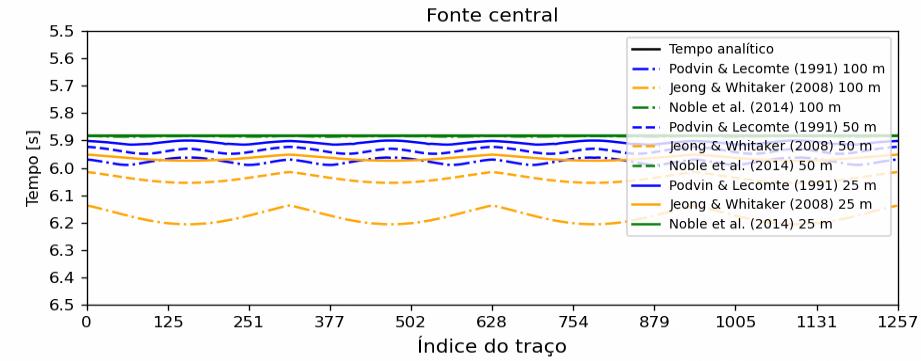
\includegraphics[width=16cm,height=6cm]{Imgs/RevisaoBibliografica/precision_direct.png}\label{fig:rnca}}\newline
	\subfloat[]{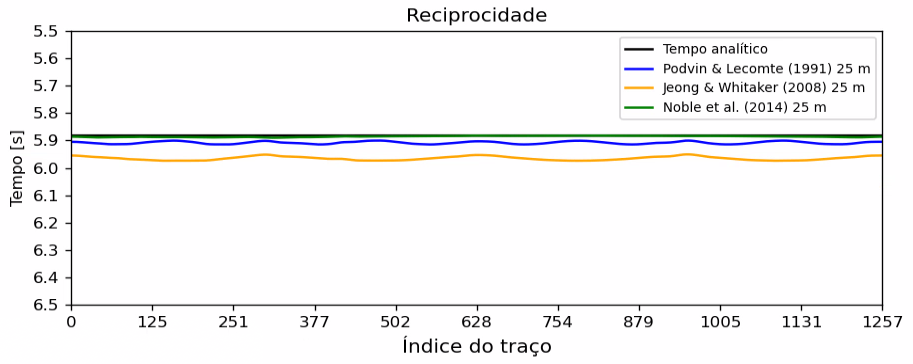
\includegraphics[width=16cm,height=6cm]{Imgs/RevisaoBibliografica/reciprocity.png}\label{fig:rncb}} 
	\caption{Panorama geral do comportamento dos tempos de trânsito para todos os métodos estudados. (a) exibe a variação para cada discretização do modelo de velocidade e (b) mostra somente o estudo de reciprocidade aplicado no modelo de 25 m.}
	\label{fig:general_refraction_study}	
\end{figure}

A solução clássica demonstrou desempenho computacional razoável para problemas pequenos, porém quando a dimensão do problema aumenta os tempos de execução não se adequam aos demais métodos. Sendo assim a formulação clássica diminui consideravelmente sua performance, no modelo com 25 m de discretização, enquanto as demais formulações mantêm seus patamares abaixo de um segundo de tempo de execução. O \textit{Fast Iterative Method} demonstrou o melhor desempenho computacional em todas as análises. Para problemas onde a precisão do cálculo dos tempos de trânsito é requerida, o \textit{Fast Iterative Method} não é tão recomendado, porém para problemas de \textit{Path Fiding} ou \textit{Shape from Shading} o método de \citeonline{jeong2008fast} é extremamente recomendável. Com a implementação em paralelo utilizando a técnica de \citeonline{detrixhe2013parallel} a variação do \textit{Fast Sweeping Method} com operadores precisos de \citeonline{noble2014accurate} demonstrou uma performance comparável ao método de \citeonline{jeong2008fast} principalmente quando aplicado no modelo de menor discretização.  

\begin{figure}[H]
	\centering
	\subfloat[]{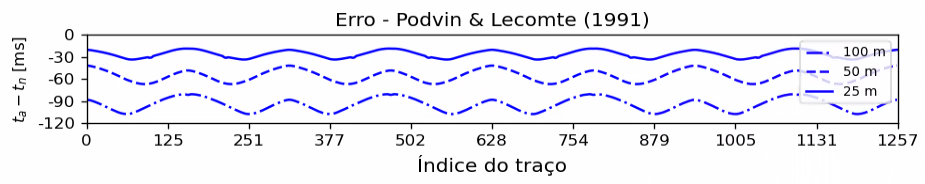
\includegraphics[width=16cm,height=3cm]{Imgs/RevisaoBibliografica/error_pod_direct.png}\label{fig:rncc}}\newline
	\subfloat[]{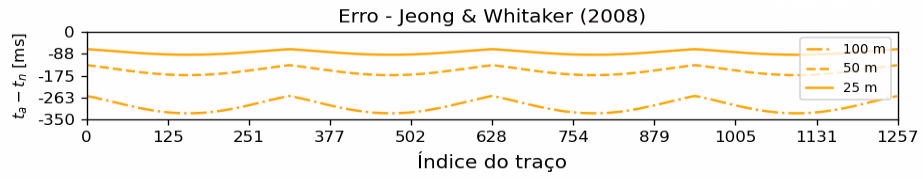
\includegraphics[width=16cm,height=3cm]{Imgs/RevisaoBibliografica/error_fim_direct.png}\label{fig:rnce}}\newline
	\subfloat[]{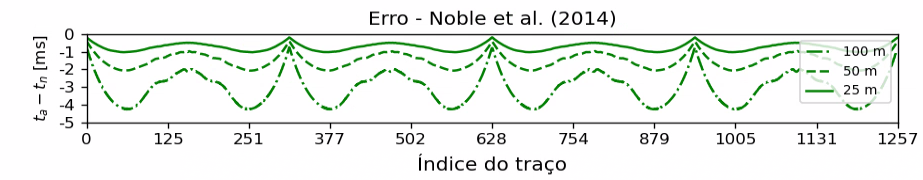
\includegraphics[width=16cm,height=3cm]{Imgs/RevisaoBibliografica/error_fsm_direct.png}\label{fig:rncg}}\newline
		
	\caption{Diferença entre os tempos analítico $t_a$ e numérico $t_n$ por método em relação aos parâmetros de discretização do modelo. (a) o método clássico de \citeonline{podvin1991finite}, (b) o FIM e (c) o FSM utilizando discretizações de 100, 50 e 25 m.}
	\label{fig:precision_refraction_study}	
\end{figure}

A Figura \ref{fig:precision_refraction_study} mostra que a diferença entre a solução analítica e a solução numérica aumentam de acordo com a esparsidade da malha, ou seja, os erros são proporcionais ao refinamento do modelo como consequência das limitações do método das diferenças finitas. A solução para melhorar a precisão é aumentar o operador de diferenças finitas para utilizar mais pontos vizinhos no cálculo dos tempos de trânsito \cite{noble2014accurate,cai2023improved}. Outra característica a se destacar na Figura \ref{fig:precision_refraction_study} são os formatos dos erros sendo periódicos de acordo com a geometria circular, causados pela formulação em coordenadas cartesianas \cite{white2020pykonal}. 

A relação de precisão entre os métodos é bem distante, sendo a formulação clássica com erros intermediários, o \textit{Fast Sweeping Method} com erros pequenos e o \textit{Fast Iterative Method} com maiores erros (Figura \ref{fig:precision_refraction_study}). Sendo assim, para problemas geofísicos, o \textit{Fast Sweeping Method} se destaca com sua performance aceitável para a precisão que proporciona, sendo o mais recomendável neste trabalho.       

\begin{figure}[H]
	\centering
	\subfloat[]{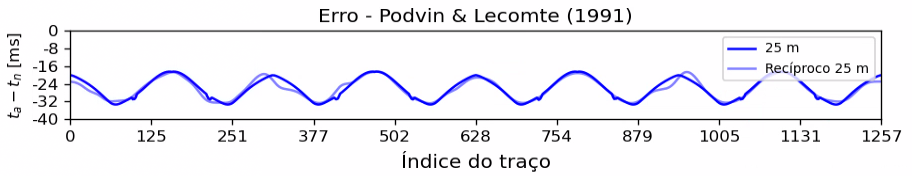
\includegraphics[width=16cm,height=3cm]{Imgs/RevisaoBibliografica/error_pod_reciprocity.png}\label{fig:rncd}}\newline
	\subfloat[]{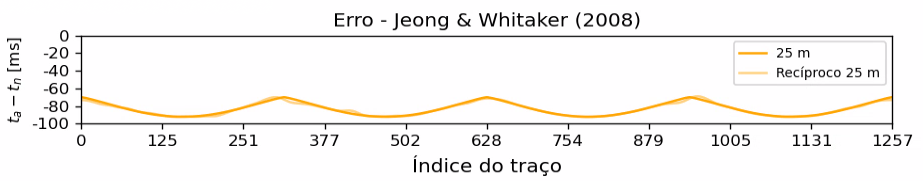
\includegraphics[width=16cm,height=3cm]{Imgs/RevisaoBibliografica/error_fim_reciprocity.png}\label{fig:rncf}}\newline
	\subfloat[]{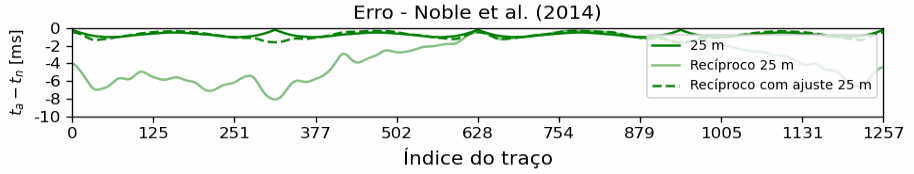
\includegraphics[width=16cm,height=3cm]{Imgs/RevisaoBibliografica/error_fsm_reciprocity.png}\label{fig:rnch}}
	
	\caption{Sobreposição entre os erros dos tempos de trânsito diretos, da fonte para os receptores, e recíprocos, dos receptores para a fonte, em relação à equação analítica. Diferença analítico $t_a$ e numérico $t_n$ em relação aos métodos (a) clássico, (b) FIM e (c) FSM somente para a discretização de 25 m entre os pontos da malha.}  
	\label{fig:reciprocity_refraction_study}
\end{figure}

A superioridade de precisão do \textit{Fast Sweeping Method} pode ser identificada também na Figura \ref{fig:reciprocity_refraction_study}, porém no estudo de reciprocidade a inicialização causou instabilidade na modelagem, como mostrado na Figura \ref{fig:reciprocity_refraction_study}c. Para iniciar o cálculo dos tempos de trânsito, todo o volume é inicializado com um valor tendendo ao infinito e somente os pontos vizinhos da fonte são inicializados com o tempo analítico para velocidade constante (equação \ref{analyticalT}). O algoritmo original de \citeonline{noble2014accurate} inicializa analiticamente somente os pontos do primeiro octante, porém o estudo de reciprocidade mostrou que a inicialização deve ser feita para os pontos vizinhos em todas as direções, ou seja,  nos oito octantes vizinhos da fonte como mostrado na Figura \ref{fig:voxel_full}. Após as correções, uma nova modelagem utilizando reciprocidade foi performada validando ainda mais a precisão do \textit{Fast Sweeping Method}, como mostrado, em linha tracejada verde, na Figura \ref{fig:reciprocity_refraction_study}c.


\section{Aplicação em modelo complexo}

As Figuras \ref{fig:overthrust_inner_circle}, \ref{fig:overthrust_mid_circle} e \ref{fig:overthrust_outer_circle} mostram os resultados gerados a partir do esquema de modelagem com geometria circular aplicado no modelo SEG/EAGE \textit{Overthrust}. Novamente as cores da figura indicam cada método, sendo a cor azul para a formulação de \citeonline{podvin1991finite}, laranja para \citeonline{jeong2008fast} e verde para a formulação de \citeonline{noble2014accurate}. As figuras são ampliações do sismograma de primeira chegada com uma seleção de estações que evidencia a disparidade entre os tempos de trânsito. Como a equação eikonal é uma aproximação da equação da onda para altas frequências, espera-se que os detalhes do modelo sejam identificados no dado, então, as janelas amplificadoras facilitam a identificação desses aspectos.    

\begin{figure}[H]
	\centering
	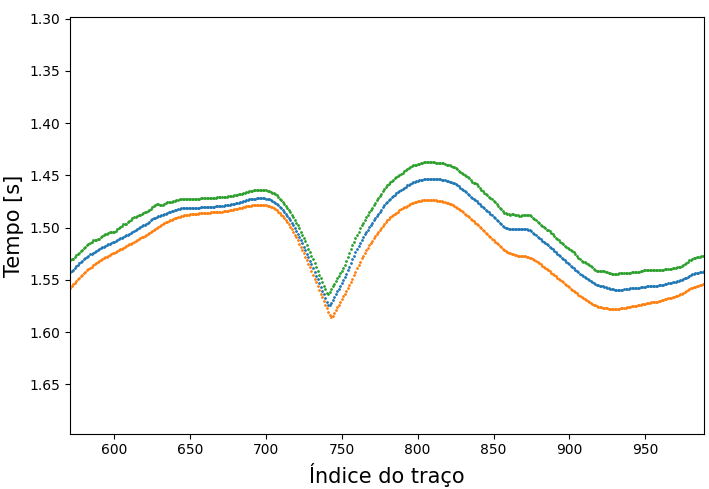
\includegraphics[height=8cm,width=13cm]{Imgs/Resultados/complex_w1.png}		
	\caption{Tempos de trânsito capturados do circulo menor de 5,5 km. As cores representam cada solução numérica, sendo azul para o método clássico, laranja para o FIM e verde para o FSM. O eixo horizontal representa o índice dos receptores entre as 5662 estações e o eixo vertical é o tempo de percurso da frente de onda.}
	\label{fig:overthrust_inner_circle}
\end{figure}

O atraso intrínseco das formulações de \citeonline{podvin1991finite} e \citeonline{jeong2008fast} pode ser notado no modelo complexo assim como foi notado utilizando o modelo simples com duas camadas. A formulação de \citeonline{noble2014accurate} se mostra superior em relação aos atrasos no tempo de trânsito por consequência dos tempos maiores observados nos demais métodos.

\begin{figure}[H]
	\centering
	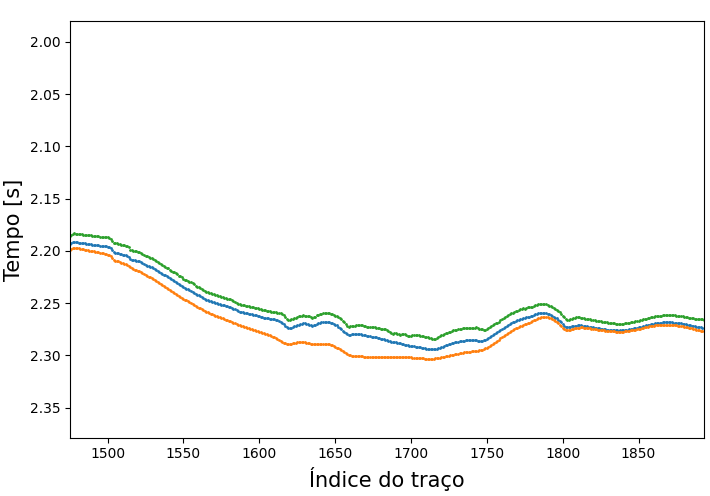
\includegraphics[height=8cm,width=13cm]{Imgs/Resultados/complex_w2.png}	
	\caption{Tempos de trânsito capturados do circulo intermediário de 7,5 km. As cores representam cada solução numérica, sendo azul para o método clássico, laranja para o FIM e verde para o FSM. O eixo horizontal representa o índice dos receptores entre as 5662 estações e o eixo vertical é o tempo de percurso da frente de onda.}
	\label{fig:overthrust_mid_circle}
\end{figure}

\begin{figure}[H]
	\centering
	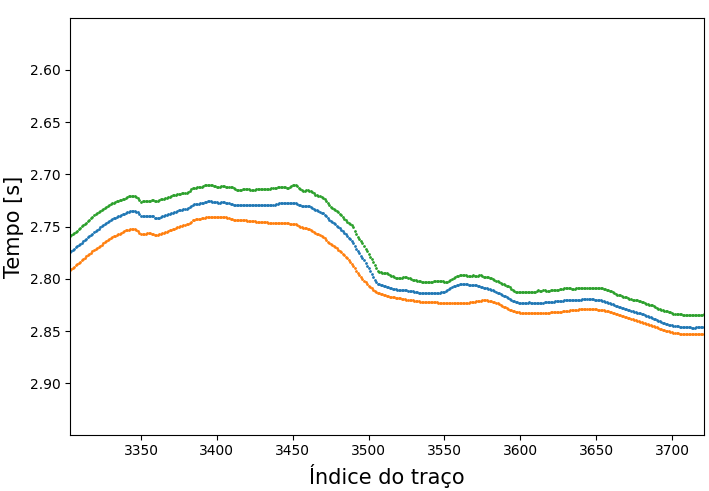
\includegraphics[height=8cm,width=13cm]{Imgs/Resultados/complex_w3.png} \newline 
	
	\caption{Tempos de trânsito capturados do círculo maior de 9,5 km. As cores representam cada solução numérica, sendo azul para o método clássico, laranja para o FIM e verde para o FSM. O eixo horizontal representa o índice dos receptores entre as 5662 estações e o eixo vertical é o tempo de percurso da frente de onda.}
	\label{fig:overthrust_outer_circle}
\end{figure}

A Tabela \ref{table_overthrust} apresenta os tempos de execução para cada método utilizando o modelo complexo em geometria circular aplicando somente um tiro no centro do modelo. A superioridade de performance é atribuída ao método de \citeonline{jeong2008fast}, porém essa metodologia possui atrasos severos em relação aos tempos de trânsito calculados comparado à equação analítica e aos demais métodos testados.

\begin{table}[H]
	\caption{Tempo de execução para a aplicação dos métodos no modelo complexo.}
	\begin{tabular}{r|c}
		& Tempo de execução \\ \hline
		\citeonline{podvin1991finite} & 11,7128 s  \\ \hline
		\citeonline{jeong2008fast} & 2,5595 s      \\ \hline
		\citeonline{noble2014accurate} & 3,4746 s         
	\end{tabular}
	\label{table_overthrust}
\end{table}

A aplicação dos métodos no modelo complexo foi realizada com sucesso, então, os tempos de trânsito (Figuras \ref{fig:overthrust_inner_circle}, \ref{fig:overthrust_mid_circle} e \ref{fig:overthrust_outer_circle}) e de execução (Tabela \ref{table_overthrust}) foram registrados. Novamente, o método clássico demonstrou tempo de execução acima dos demais para problemas grandes. O método de \citeonline{jeong2008fast} demonstra eficiência computacional e o \textit{Fast Sweeping Method} performa 26$\%$ abaixo do método mais performático. Considerando o ganho de precisão, a diferença de performance pode ser desconsiderada pois \citeonline{cai2023improved} mostram a utilização do método original de \citeonline{jeong2008fast} na migração Kirchhoff em profundidade, onde os erros de posicionamento dos refletores são amplamente perceptíveis. Os tempos de trânsito ilustrados nas Figuras \ref{fig:overthrust_inner_circle}, \ref{fig:overthrust_mid_circle} e \ref{fig:overthrust_outer_circle} mostram as discrepâncias entre os métodos aplicados ao modelo SEG/EAGE \textit{Overthrust}, sendo que os atrasos percebidos na Figura \ref{fig:precision_refraction_study} se repetem, porém no modelo complexo. Se mostra visível nas Figuras \ref{fig:overthrust_inner_circle}, \ref{fig:overthrust_mid_circle} e \ref{fig:overthrust_outer_circle} os detalhes que o modelo impõe aos tempos de trânsito, nas formulações de \citeonline{podvin1991finite} e \citeonline{noble2014accurate}, e a falta de definição para a formulação menos precisa de \citeonline{jeong2008fast}.  





